

\documentclass[a4paper,11pt]{article} 
\usepackage[spanish]{babel}           
\usepackage[utf8]{inputenc}           

\usepackage[T1]{fontenc}   		   % Fonte por defecto.
\usepackage{graphicx, subfigure}    		   % Engadir imaxes.
\usepackage{color}      		   % Uso de cores.
\usepackage{anysize}     		   % Modificar o tamaño dos marxes.
\usepackage{multicol, multirow}    % Escribir a doble, triple...columna.
\usepackage{bm}          		   % Letras gregas en negriña.
\usepackage{textcomp}    		   % Símbolos, poden consultarse na rede.
\usepackage{eurosym}     		   % Símbolo € (\euro).
\usepackage{amsthm}                % Paquete da AMS para escribir teoremas.
\usepackage{amsmath,amsfonts}      %Paquetes específicos de símbolos.
\usepackage{lineno}                % Numerar as liñas.
\usepackage{fancyhdr}

\marginsize{1.5cm}{1.5cm}{1.5cm}{1.5cm} % MARXES: Esq, der, sup, inf.
\parindent=7mm                        % Sangría. 
\parskip=2mm                          % Espazo entre párrafos.
\renewcommand{\baselinestretch}{1}    % Interliñado.


\title{Título do artigo}
\author{}
\date{} %Para que non apareza deixa o espaxo entre {} valeiro. Para que apareza a data de hoxe: \today


\begin{document}  


\maketitle 
\thispagestyle{empty}  
  
\newpage
\thispagestyle{empty}     
\tableofcontents  % Índice.


\newpage
\setcounter{page}{1}   

\pagestyle{fancy}
\lhead{}
\rhead{Memoria y emoción}
\cfoot{\thepage}

\section{Resumen}
A partir de este trabajo se pretende verificar la idea de Bower de que se recuerda mejor aquello que es congruente con el estado de ánimo. Para ello, y partiendo de estudios anteriores de otros autores como Guerrero et al., se ha evaluado a través de un inventario el grado de depresión de 149 estudiantes de Psicología que cursan la asignatura de Memoria,  para después relacionar los resultados obtenidos para cada uno de los sujetos experimentales con el número de palabras recordadas por cada uno de ellos (positivas, negativas y neutras) en una prueba de memoria. 

Empleamos un total de 52 palabras, siendo el número de palabras con valor emocional neutro el doble que el de el resto de palabras: así, se utilizaron 26 palabras neutras, 13 positivas y 13 negativas. Los resultados obtenidos demuestran la existencia de una relación entre cognición y emoción que permite verificar la idea de Bower(1981), ya que los resultados que se esperan de los sujetos depresivos (más de 15 puntos en el inventario Depresión de Beck) reconozcan con más facilidad palabras negativas que las positivas en una tarea de reconocimiento.  

En este sentido, hemos encontrado en nuestros sujetos que el recuerdo de palabras negativas resulta ser altamente significativo frente al número de palabras de índole positiva y neutra. Así mismo, se han encontrado un buen número de falsas alarmas, aunque no hemos concluído que sean significativas. 

\vspace{1cm}

\textbf{PALABRAS CLAVE:} Emoción, recordar, depresión, palabras, estado de ánimo. 

\section{Introducción}
La memoria es el proceso neurocognitivo que permite registrar, codificar, consolidar, almacenar, acceder y recuperar la información. En su funcionamiento influyen elementos fisiológicos: por ejemplo, una lesión en el hipocampo puede alterar la capacidad para crear nuevos recuerdos. El estado emocional de la persona también influye considerablemente en la memoria; cuando una emoción se prolonga en el tiempo se convierte en un estado de ánimo, por lo que influye en la toma de decisiones e incluso puede alterar algunas funciones cerebrales. Diversos equipos de expertos llevan mucho tiempo estudiando cómo afecta la emoción a nuestro cerebro desde distintos enfoques, desde la psicología cognitiva del siglo XX hasta la más actual apuesta por la neuropsicología (J.R.Caballero).

Se suele decir que la cognición causa la aparición de los estados emocionales en las personas; sin embargo, este siempre ha sido un tema que ha causado polémica a lo largo de la historia de la psicología. En este trabajo trataremos este tema partiendo del estudio de Guerrero.

Guerrero et al. parten de la idea de Bower de que cada uno de los estados emocionales produce un efecto congruente con dicho estado. Es decir, que un estado de ánimo depresivo produce un recuerdo relacionado con este estado afectivo, y viceversa. Bower defendía, además, la existencia de nodos que se activan cuando un sujeto se encuentra bajo un estado de ánimo determinado, facilitando así el recuerdo de sucesos y pensamientos que se han ido aprendiendo poco a poco. Por otra parte, al facilitar el recuerdo relacionado con una determinada emoción, se inhibirá el recuerdo de los nodos que senn incongruentes ella. 

Con toda esta información, Guerrero et al. realizan un trabajo cuyo propósito es estudiar la influencia de los estados emocionales de alegría y tristeza a través de la codificación y recuperación de palabras relacionadas con estos dos estados. Para ello presentan a los sujetos imágenes y música relacionadas con ambos estados. Este trabajo reafirma la concepción de Bower sobre la relación existente entre cognición y emoción, y pone de manifiesto la importancia de los fenómenos emocionales sobre los cognitivos. Además, ahora sabemos que el estado de ánimo no sólo influye en el recuerdo: otros trabajos han demostrado que este también está relacionado con la codificación y la percepción.

En esta línea, Brown y Kulik establecen la existencia de una memoria emocional que almacena aspectos relacionados con las emociones, permitiendo así explicar por qué es más fácil recordar aquellas circunstancias que poseen más implicaciones afectivas. Tras este estudio empieza a ser necesario diferenciar entre memoria emocional y memoria de la emoción. La primera se encuentra mediada por la amígdala, y la segunda, por el hipocampo.  Esta última es, además, una memoria declarativa. Ambas operan en paralelo y es posible que almacenen información distinta.

Aunque, como aclaramos antes, nosotras hemos realizado este informe basándonos en trabajo de Guerrero et al. (2010), existen otros muchos trabajos relacionados con este tema. Por ejemplo, el trabajo realizado por Redondo, Fraga, Comesaña y Perea, en el que se encontró, tras realizar numerosos análisis verbales, que la varianza de las evaluaciones se puede explicar en dos dimensiones, activación y valencia, utilizando para ello el Maniquí de Autoevaluación (SAM). 

\section{Método}
\subsection{Participantes}
Para la realización de esta práctica hemos utilizado una muestra de 149 estudiantes de diferentes edades que cursan el segundo año del Grado en Psicología de la Universidad de Santiago de Compostela (USC), y en cuyo programa se incluye la materia de Psicología de la Memoria. Los hemos dividido en grupos de veinte personas, aproximadamente.

\subsection{Materiales y procedimiento}
Los materiales que hemos empleado han sido:
\begin{itemize}
	\item[•] Inventario de Depresión de Beck (BDI)
	\item[•] Listado de palabras emocionalmente positivas, negativas y neutras, confeccionado a
	partir del estudio de Redondo et al.(2005)
	\item[•] Tarea distractora con figuras
	\item[•] Resultados de los ocho grupos de prácticas
\end{itemize}

Para llevar a cabo el experimento, se pasó el inventario de de Depresión de Beck (BDI, Beck, Rush, Shaw y Emery, 1979) a todos los estudiantes en el aula, divididos en grupos de unas veinte personas según el orden alfabético de sus primeros apellidos. Dicho inventario, creado por el psiquiatra, investigador y fundador de la Terapia cognitiva, Aaron T. Beck, (1983) es un cuestionario autoadministrado que consta de veintiún ítems con cuatro opciones de respuesta, de las cuales debe elegirse sólo una. Es uno de los instrumentos más comúnmente utilizados para medir la severidad de una depresión. Está compuesto por ítems relacionados con síntomas depresivos, como la desesperanza o la irritabilidad, con cogniciones como culpa o con sentimientos como estar siendo castigado, así como con síntomas físicos relacionados con la depresión (fatiga, pérdida de peso y de apetito sexual, etc.).
 
Tras la cumplimentación del inventario, cada alumno ha podido sumar los valores asignados a cada una de sus respuestas. Así se han obtenido las puntuaciones de cada test, donde:
\begin{itemize}
	\item[-] Tener una puntuación inferior a 15 puntos implica ser una persona no depresiva.
	\item[-] Tener una puntuación superior a 15 puntos implica padecer algún grado de depresión. Se
	supone, además, que las puntuaciones superiores a 30 puntos alertan de un posible problema grave
	de depresión.
\end{itemize}

Esta diferenciación es muy importante porque nos ayudara, más tarde, a determinar si se cumple la hipótesis de que las personas con depresión recuerdan mejor las palabras negativas.

Justo después de haber respondido al cuestionario se les ha leído a los sujetos un listado de palabras emocionalmente positivas, negativas y neutras, elaborado a partir del estudio de Redondo et al. (2005). Del total de palabras, veintiséis eran neutras, trece eran positivas y otras trece eran negativas.

A continuación se les ha pedido a los sujetos que realizasen una tarea distractora, consistente en buscar unos tipos concretos de flechas entre un patrón lleno de ellas. Tras unos minutos se finalizó con la tarea y se les entregó a los sujetos un listado de palabras, de entre las cuales debían seleccionar aquellas que recordaban haber oído durante la lectura de la primera lista.

En esta parte del experimento es muy probable que los sujetos seleccionen en la lista algunas palabras que creen haber oído aunque en realidad no lo han hecho. Estas son las llamadas falsas alarmas, casos o circunstancias en las que estamos seguros de poseer recuerdos veraces sobre ciertos eventos que en realidad nunca nos han pasado, o no han ocurrido en realidad. Las memorias falsas son importantes porque constituyen una prueba de que los recuerdos contenidos en la memoria no son una copia literal del pasado, sino que dependen de procesos constructivos que pueden estar llenos de errores, distorsiones e incluso ilusiones. Lo importante de las falsas memorias es que son características del recuerdo normal, más que del recuerdo patológico. Uno de los ejemplos más estudiados sobre el reconocimiento falso surge a partir de los estudios de Elizabeth Loftus (1995).

Por último se llevó a cabo la suma de todas las palabras seleccionadas, clasificándolas en positivas, negativas y neutras. Se hizo esto para las palabras que estaban en la primera lista (aciertos) y para las que no lo estaban (falsas alarmas). Por último, se colocaron los resultados de cada grupo en una tabla común para su posterior análisis.

\subsection{Análisis}
Para el análisis de los resultados se han empleado una serie de estadísticos descriptivos, separando a los sujetos en dos grupos: depresivos y no depresivos. Además, en cuanto a los aciertos positivos, negativos y neutros se ha calculado la significación para cada uno, comparando al grupo de sujetos depresivos con el de sujetos no depresivos.

Por otro lado, para las falsas alarmas en cada grupo se han obtenido los estadísticos descriptivos media y desviación típica, con los que se ha obtenido posteriormente la significación de las puntuaciones. 

La variable independiente en este experimento ha sido el estado anímico de los sujetos, y la dependiente, el número de palabras (aciertos y falsas alarmas) seleccionado por cada uno de ellos en base a sus recuerdos.

\section{Resultados}

\begin{table}[h!]
\centering
\begin{tabular}{l|c|c|c|c|c|c|}
\cline{2-7}
                                        & \multicolumn{3}{c|}{No depresivos}                                                                                                                                                                               & \multicolumn{3}{c|}{Depresivos}                                                                                                                                                                                  \\ \cline{2-7} 
                                        & \begin{tabular}[c]{@{}c@{}}Falsas\\ alarmas\\ positivas\end{tabular} & \begin{tabular}[c]{@{}c@{}}Falsas\\ alarmas\\ negativas\end{tabular} & \begin{tabular}[c]{@{}c@{}}Falsas\\ alarmas\\ neutras\end{tabular} & \begin{tabular}[c]{@{}c@{}}Falsas\\ alarmas\\ positivas\end{tabular} & \begin{tabular}[c]{@{}c@{}}Falsas\\ alarmas\\ negativas\end{tabular} & \begin{tabular}[c]{@{}c@{}}Falsas\\ alarmas\\ neutras\end{tabular} \\ \hline
\multicolumn{1}{|c|}{Media}             & 0.69                                                                 & 0.85                                                                 & 0.89                                                               & 0.74                                                                 & 0.93                                                                 & 0.93                                                               \\ \hline
\multicolumn{1}{|c|}{Desviación típica} & 0.27                                                                 & 0.41                                                                 & 0.41                                                               & 0.42                                                                 & 0.45                                                                 & 0.32                                                               \\ \hline
\end{tabular}
\caption{Estadísticos descriptivos para las falsas alarmas}
\end{table}

\begin{table}[h!]
\centering
\begin{tabular}{c|c|c|c|c|c|c|}
\cline{2-7}
\multicolumn{1}{l|}{}                   & \multicolumn{3}{c|}{No depresivos}                                                                                                                                                       & \multicolumn{3}{c|}{Depresivos}                                                                                                                                                          \\ \cline{2-7} 
\multicolumn{1}{l|}{}                   & \begin{tabular}[c]{@{}c@{}}Aciertos\\ positivos\end{tabular} & \begin{tabular}[c]{@{}c@{}}Aciertos\\ negativos\end{tabular} & \begin{tabular}[c]{@{}c@{}}Aciertos\\ neutros\end{tabular} & \begin{tabular}[c]{@{}c@{}}Aciertos\\ positivos\end{tabular} & \begin{tabular}[c]{@{}c@{}}Aciertos\\ negativos\end{tabular} & \begin{tabular}[c]{@{}c@{}}Aciertos\\ neutros\end{tabular} \\ \hline
\multicolumn{1}{|c|}{Media}             & 7.88                                                         & 7.33                                                         & 14.83                                                      & 8.09                                                         & 8.84                                                         & 15.19                                                      \\ \hline
\multicolumn{1}{|c|}{Desviación típica} & 0.58                                                         & 0.65                                                         & 1.07                                                       & 1.03                                                         & 0.80                                                         & 2.34                                                       \\ \hline
\multicolumn{1}{|c|}{Porcentajes}       & 60.62                                                        & 56.38                                                        & 57.04                                                      & 62.23                                                        & 68                                                           & 58.42                                                      \\ \hline
\multicolumn{1}{|c|}{Error típico}      & 0.21                                                         & 0.33                                                         & 0.38                                                       & 0.36                                                         & 0.28                                                         & 0.83                                                       \\ \hline
\multicolumn{1}{|c|}{Límite\footnotemark superior}   & 8.28                                                         & 7.78                                                         & 15.57                                                      & 8.80                                                         & 9.40                                                         & 16.81                                                      \\ \hline
\multicolumn{1}{|c|}{Límite inferior}   & 7.48                                                         & 6.88                                                         & 14.09                                                      & 7.38                                                         & 8.28                                                         & 13.57                                                      \\ \hline
\multicolumn{1}{|c|}{Mínimo}            & 6.71                                                         & 6.26                                                         & 13.53                                                      & 6.83                                                         & 7.25                                                         & 11.43                                                      \\ \hline
\multicolumn{1}{|c|}{Máximo}            & 8.69                                                         & 8.44                                                         & 16.58                                                      & 9.6                                                          & 9.62                                                         & 19                                                         \\ \hline
\end{tabular}
\caption{Estadísticos descriptivos de los aciertos}
\end{table}

La significación de falsas alarmas para ambos grupos (depresivos y no depresivos) ha sido superior a 0.25 en los tres casos (positivas, negativas y neutras). Por tanto, concluimos que las falsas alarmas en nuestra replicación del experimento no son significativas.

Por otra parte, la significación tanto de aciertos positivos como de aciertos neutros también ha superado el 0.25, por lo que los resultados obtenidos en estas categorías no son significativos para ninguno de los dos grupos. Sin embargo, la significación obtenida para los aciertos negativos es inferior al 0.05, lo cual indica que nuestros resultados, en este caso, son altamente significativos.

\footnotetext{Intervalo de confianza 95\% para la media}

\section{Discusión}
Los resultados encontrados en este experimento indican, en primer lugar, que los sujetos depresivos, en comparación con los del grupo no depresivo, presentan en la prueba de recuerdo libre un peor recuerdo independiente del tipo estímulo presentado. Estos datos son consistentes con los resultados obtenidos en estudios previos (e.g., Calev y Erwin, 1985; Hart, Kwentus, Hamer y Taylor, 1987), que indican que los sujetos depresivos muestran un déficit de memoria respecto a los sujetos no depresivos en tareas de recuerdo libre. 

Por otro lado, los resultados también indican que las personas con tendencias depresivas recuerdan más palabras negativas que positivas y neutras. O lo que es lo mismo, los pacientes depresivos tienen un sesgo de recuerdo negativo, consistente en la tendencia a recordar selectivamente aquellas palabras que son congruentes con su estado de afectivo. A nivel empírico, estos resultados coinciden con otros obtenidos en estudios de la misma índole (e.g., Clark y Teasdale, 1985, exp. 1; Ruiz-Caballero y Bermúdez, 1993; Ruiz-Caballero y Donoso-Cortés, 1999). A nivel teórico, son consistentes con las hipótesis derivadas del modelo de red asociativa de la emoción de Bower (1981), que predice que el estado de ánimo tiende a producir un efecto de recuerdo congruente con él. 

Podemos observar, también, que el efecto de recuerdo congruente con el estado de ánimo no aparece para las palabras positivas. Esto sugiere que dicho efecto de congruencia puede ser explicado mediante la activación de constructos negativos específicos, que facilitan el acceso a las experiencias negativas y son responsables del recuerdo selectivo de la información negativa. 

El modelo de Bower (1981) se caracteriza por el uso de tareas sencillas, en las que se presentan estímulos simples (normalmente palabras) de contenido afectivo negativo o positivo, y por la posterior evaluación de dichas tareas mediante pruebas de recuerdo intencional o incidental (tareas de recuerdo libre y/o reconocimiento). Por este motivo, es posible que los sesgos de memoria congruentes con el estado de ánimo puedan ser explicados en base a los cambios producidos en los modelos mentales que se emplean para interpretar la información, especialmente cuando la información se presenta en unidades lingüísticas más largas que las palabras y están relacionadas con deseo personal de aprobación social. 

Sin embargo, cuando simplemente se utilizan palabras emocionales aleatorias (no relacionadas con la aprobación social o el logro personal), los datos sugieren que el efecto de recuerdo congruente con el estado de ánimo puede explicarse en términos de accesibilidad o activación de los mencionados constructos negativos específicos.

\section{Conclusiones}
Como hemos visto, el estado de ánimo es un potente modulador de los procesos psicológicos básicos que ocurren en la mente humana. Un procesamiento de la información negativo puede hacer que aparezcan determinados sesgos que provoquen que la atención, la percepción y la memoria se vean afectados. 

La memoria contiene un importante arsenal de experiencias y recuerdos pasados que sirven de proyección futura para llevar a cabo numerosos comportamientos en nuestro día a día, entre otras funciones. En este sentido, se conoce que la depresión puede hacer que el número de recuerdos específicos positivos se vean mermados, en comparación con un estado de ánimo no depresivo o eutímico. Estos datos van enlazados con el Modelo de Red Asociativa de Bower (1981), que muestra cómo los estados de ánimo depresivos incrementan la activación y accesibilidad de cogniciones negativas, fruto del ya mencionado efecto de congruencia.

Según este modelo, cada estado emocional estaría representado por un nodo emocional, dentro de una red cognitiva de trazos de memoria relacionados con dicho estado. Al activarse el nodo emocional se evocan estas cogniciones y trazos de memoria, y es esto lo que facilita que la información afectiva congruente con el estado de ánimo del individuo tienda a ser mejor codificada que la información afectivamente incongruente. 

Nuestros resultados confirman, en parte, las hipótesis expuestas: a mayor puntuación en el cuestionario  de Beck, mayor recuerdo de palabras negativas. Los alumnos con supuestas tendencias depresivas (es decir, cuya puntuación es superior a quince) recuerdan de forma significativamente mejor las palabras negativas que las positivas. 

La media para el número de aciertos en sujetos no depresivos es significativamente mayor que la media para falsas alarmas de este mismo grupo. Lo mismo ocurre con los sujetos depresivos. A su vez, si comparamos la media de aciertos en el grupo de sujetos depresivos con la media de aciertos en el grupo de los no depresivos, vemos que los primeros obtienen medias superiores.

En cuanto a los sujetos no depresivos, podemos observar, como se esperaba, que su media de aciertos positivos es superior a la obtenida en los aciertos negativos. Sin embargo, no puede afirmarse que esta diferencia sea significativa. Los resultados demuestran que el recuerdo de palabras negativas en sujetos depresivos es significativo, al contrario que en los no depresivos, donde el recuerdo de palabras positivas no es en absoluto significativo.

Por último, si nos detenemos a observar las falsas alarmas, podemos observar que el recuerdo de falsas alarmas negativas es ligeramente mayor en los sujetos depresivos, pero no ocurre lo mismo con el de falsas alarmas positivas en sujetos no depresivos. De nuevo, estos resultados no son significativos, por lo que podemos concluir que las falsas alarmas no han aportado información reveladora a nuestro trabajo.

\newpage

\section{Referencias bibliográficas}
\indent

\leftskip 0.3in
\parindent -0.3in

Beck, A. T., Rush, A. J., Shaw, B. F., y Emery, G. (1983). \textit{Terapia cognitiva de la depresión.} Brouwer.

Bower, G. H. (1976). \textit{Los modelos del procesamiento de la información.} Hilgard ER y GH Bower, Teorías del aprendizaje. México: Edit. Trillas.

Cabaco, A. S., León, A. C., y Martínez, J. M. A. (2014). \textit{Prácticas de psicología de la memoria.} Alianza Editorial.

Cabeza Peribáñez, C. B., Sánchez Cabaco, A., y Urchaga Litago, D. (2014). \textit{Memoria autobiográfica y estado de ánimo: estudio empírico-diferencial en mayores y jóvenes.}

Guerrero, C., Meilán, J. J. G., Carpi, A., y Palmero, F. (2008). Capítulo 8. Emoción y memoria: influencia del estado afectivo en el proceso de reconocimiento de palabras.  \textit{Emoción y motivación: Contribuciones actuales} (vol. I, pp. 109-118). San Sebastián: Mitxenela.

 Meilán G.,  Carro, J., Guerrero, C., Carpi, A., Gómez, C., y Palmero, F. (2012). El efecto de memoria congruente con el estado afectivo: reconocimiento diferencial de palabras de tristeza y alegría. \textit{Anales de psicologia, 28}(1).
 
Loftus, E. F., y Pickrell, J. E. (1995). The formation of false memories. \textit{Psychiatric annals, 25}(12), 720-725.

Redondo, J., Fraga, I., Comesaña, M., y Perea, M. (2005). Estudio normativo del valor afectivo de 478 palabras españolas. \textit{Psicológica, 26}(2).

Ruiz Caballero, J. A., y Sánchez Arribas, C. (2001). Depresión y memoria: ¿Es la información congruente con el estado de ánimo más accesible? \textit{Psicothema, 13}(2).

\newpage

\section{Anexo I: Gráficos}
\begin{figure}[h!]
	\centering
	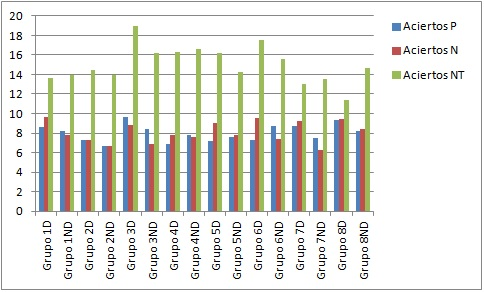
\includegraphics[width=0.55\linewidth]{informe1_1}
	\caption{Aciertos para cada grupo de sujetos}
\end{figure}

\begin{figure}[h!]
	\centering
	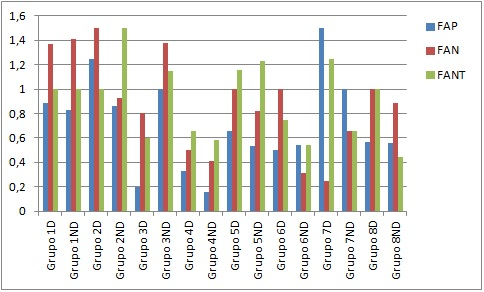
\includegraphics[width=0.55\linewidth]{informe1_2}
	\caption{Falsas alarmas para cada grupo de sujetos}
\end{figure}

\begin{figure}[h!]
	\centering
	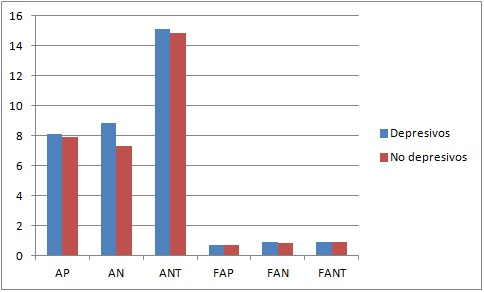
\includegraphics[width=0.55\linewidth]{informe1_3}
	\caption{Resultados para sujetos depresivos y no depresivos}
\end{figure}

\newpage

\section{Anexo II: Tablas}
\begin{table}[h!]
\centering
\begin{tabular}{|c|c|c|c|c|c|c|c|}
\hline
                         &    & AP   & AN   & ANT   & FAP  & FAN  & FANT \\ \hline
\multirow{2}{*}{Grupo 1} & Depresivos  & 8.62 & 9.62 & 13.62 & 0.89 & 1.37 & 1    \\ \cline{2-8} 
                         & No depresivos & 8.17 & 7.66 & 13.91 & 0.83 & 1.41 & 1    \\ \hline
\multirow{2}{*}{Grupo 2} & Depresivos  & 7.25 & 7.25 & 14.5  & 1.25 & 1.5  & 1    \\ \cline{2-8} 
                         & No depresivos & 6.71 & 6.71 & 13.93 & 0.86 & 0.93 & 1.5  \\ \hline
\multirow{2}{*}{Grupo 3} & Depresivos  & 9.6  & 8.8  & 19    & 0.2  & 0.8  & 0.6  \\ \cline{2-8} 
                         & No depresivos & 8.38 & 6.85 & 16.23 & 1    & 1.38 & 1.15 \\ \hline
\multirow{2}{*}{Grupo 4} & Depresivos  & 6.83 & 7.83 & 16.33 & 0.33 & 0.5  & 0.66 \\ \cline{2-8} 
                         & No depresivos & 7.75 & 7.58 & 16.58 & 0.16 & 0.41 & 0.58 \\ \hline
\multirow{2}{*}{Grupo 5} & Depresivos  & 7.16 & 9    & 16.16 & 0.66 & 1    & 1.16 \\ \cline{2-8} 
                         & No depresivos & 7.6  & 7.76 & 14.23 & 0.53 & 0.82 & 0.54 \\ \hline
\multirow{2}{*}{Grupo 6} & Depresivos  & 7.25 & 9.5  & 17.5  & 0.5  & 1    & 0.75 \\ \cline{2-8} 
                         & No depresivos & 8.69 & 7.39 & 15.54 & 0.54 & 0.31 & 0.66 \\ \hline
\multirow{2}{*}{Grupo 7} & Depresivos  & 8.75 & 9.25 & 13    & 1.5  & 0.25 & 1.25 \\ \cline{2-8} 
                         & No depresivos & 7.53 & 6.26 & 13.53 & 1    & 0.66 & 0.66 \\ \hline
\multirow{2}{*}{Grupo 8} & Depresivos  & 9.29 & 9.43 & 11.43 & 0.57 & 1    & 1    \\ \cline{2-8} 
                         & No depresivos & 8.22 & 8.44 & 14.67 & 0.56 & 0.89 & 0.44 \\ \hline
\end{tabular}
\caption{Medias para cada grupo de sujetos en cada categoría}
\end{table}

\end{document} %Non pode haber nada escrito despois desta instrución.
